% define documentclass
\documentclass[12pt, bibliography=totoc, a4paper, abstractoff, numbers=noenddot]{scrreprt}

% define used packages
\usepackage[left=4.0cm, right=2.0cm, top=3cm, bottom=3cm]{geometry}
%\usepackage{bibgerm}
\usepackage{babelbib}
\usepackage[utf8]{inputenc}
\usepackage[T1]{fontenc}
\usepackage{graphicx}
\usepackage[ngerman]{babel}
\usepackage{lmodern}
\usepackage{listings}
\usepackage[numbers]{natbib}
\usepackage{acronym}
\bibliographystyle{alphadin}
\usepackage{float}
\usepackage[title]{appendix}

\usepackage{lastpage}

% advanced tables
\usepackage{array}

% header and footer
\usepackage{fancyhdr}

% links
\usepackage{url}

% internal links
\usepackage[colorlinks=true ,linkcolor=black,
			anchorcolor=black ,citecolor=black ,filecolor=black,
			menucolor=black ,urlcolor=black]{hyperref}

% mathematical formulas
\usepackage{amsmath, amssymb}

% fancy Diagrams %
\usepackage{tikz}
\usepackage{epstopdf}

% to include images side by side
\usepackage{subfigure}

% for nice bg on title page
\usepackage{eso-pic}
\newcommand\BackgroundPic{%
\put(0,0){%
\parbox[b][\paperheight]{\paperwidth}{%
\vfill
\centering
\includegraphics[width=\paperwidth,height=\paperheight,%
keepaspectratio]{images/Logo_H-BRS_background}%
\vfill
}}}

% define the programming language
\input{lststyles}

%set default pagestyle
\pagestyle{empty}


\setlength{\parindent}{0pt}
\setlength{\parskip}{12pt}

% #####
% #
% # START config area
% #
% #####

\newcommand{\HEADER}[0]{H-BRS, WS 2016 / 2017}
\newcommand{\PAGENUMBERS}[0]{\pagemark}
\newcommand{\DATE}[0]{12.10.2016}

\newcommand{\AUTHOR}[0]{Johann Martens, Moritz Kemp}
\newcommand{\MATNR}[0]{}
\newcommand{\STREET}[0]{}
\newcommand{\ZIP}[0]{}
\newcommand{\TOWN}[0]{}

\newcommand{\REFERENT}[0]{Prof. Dr. Harm Knolle}
%\newcommand{\KOREFERENT}[0]{}

\newcommand{\TITLE}[0]{Aufbau einer NoSQL-Datenbank mit Apache Hadoop und Apache HBase für das Million Song Dataset}
\newcommand{\COURSE}[0]{Schemalose Datenbanken}
\newcommand{\TYPE}[0]{Semester-Projekt}
\newcommand{\COMPLETION}[0]{}

% #####
% #
% # END config area
% #
% #####

% Hurenkinder und Schusterjungenregelung
\clubpenalty=100000
\widowpenalty=100000
\displaywidowpenalty=100000

% starting the document
\begin{document}

% set pagenumbering to roman(I II III IV)
\pagenumbering{Roman}
% input the title
\input{title}

\begin{abstract}
\section*{Zusammenfassung}\markboth{Zusammenfassung}{}
  \addcontentsline{toc}{chapter}{Zusammenfassung}
  Das Ziel der Projektarbeit zum Thema \textit{Hadoop/Hbase} ist es, 
eine Datenbank mittels Hadoop/Hbase auf einem bereitgestelltem
Cluster so zu installieren, dass der Anwender in dem One-Million-Datensatz nach Liedern
suchen kann. 
Im ersten Teil der Projektarbeit werden die theoretischen Grundlagen von Hadoop/Hbase 
behandelt. Dazu gehört ein Kapitel zu Map/Reduce, ein Kapitel zu Hadoop und ein Kapitel zu Hbase.
Die Theorie soll etwa ein Drittel der Projektarbeit ausmachen. 

Der zweite Teil der Projektarbeit, zwei Drittel der Projektarbeit, beschreibt die praktische Umsetzung, die aus der Installation und 
Konfiguration der Hadoop/Hbase-Datenbank und der Implementierung der Client-Software besteht.
Eingangs werden Anforderungen, Anwendungsfälle und technische Rahmenbedingungen kurz beschrieben,
um einen Überblick zu geben. Anschließen folgen das Kapitel der Installation bzw. Implementierung von
Hadoop/Hbase auf den Clustern. Hier wird das Vorgehen  beschrieben, wie die Installation und Konfiguration 
abläuft. Eingesetzte Programmiersprachen sind hier Java und JRuby. Fragestellungen werden sein, wie 
sich die Datenbank auf einen Cluster installieren lässt und welche Konfigurationsparameter hinsichtlich des
Anwendungsfalls eines One-Million-Datensatzes berücksichtigt und angepasst werden müssen. Auch die konkrete
Implementierung der map und reduce Funktionen wird in diesem Kapitel dargelegt. Auch FIlter- und Optimierungsparameter,
die besonders Hbase betreffen, werden evaluiert und gegebenenfalls angewendet.
Zum Abschluss wird gezeigt,
ob und wie sich die Datenbank auch ohne eigens programmiertem Client Ad-Hoc ansprechen lässt, beispielsweise über
eine laufende Shell. Das nächste Kapitel beschreibt die Implementierung der Client-Software, die mittels Java als Serveranwendung
und Javascript als Client-Anwendung dem Anwender die Möglichkeit bieten soll, über eine grafische Oberfläche mit dem One-Million-Datensatz
zu arbeiten. Der Client hat dabei aber wenige, nur funktionale Anforderungen, eine aufwendig grafische Oberfläche ist nicht das Ziel.
Ein weiteres Kapitel im praktischen Teil behandelt die Installation des One-Million-Datensatzes in das Hadoop-Dateisystem.
Wichtige Fragestellungen spielt dabei, inwieweit die Daten bereits für die Speicherung im Hadoop-Dateisystem geeignet sind 
sowie die Frage nach der Replikation auf dem Cluster-System.

Zum Abschluss des praktischen Teils folgt eine kurze Leistungsdarstellung des Systems, indem die Antwortzeiten
der Datenbank zu bestimmten Abfragen gemessen werde. Optional ist eine Leistungsbewertung im Vergleich mit 
den anderen Teams denkbar, die ebenfalls mit dem selben Datensatz arbeiten.

%Das Team wird sich zuerst mit den Grundlagen von NoSQL-Datenbanken befassen, 
%vor allem explizit mit den Grundlagen von Hadoop/Hbase. Darauf aufbauend lässt
%sich eine Argumentation formulieren, warum sich die Behandlung von derart großen Datensätzen
%wie dem Million-Song-Datensatz mit Hadoop/Hbase effektiver gestalten lässt als mit klassischen relationalen Datenbanken. Dieser Teil beinhaltet also im wesentlichen
%Grundlagen zu den Wide-Column-Datenbanken sowie Grundlagen zu Hadoop und Hbase.

%Im praktischen Teil wird zunächst die benötigte Software installiert, i.e. Java, Hadoop und HBase. Um die Installation auf einer Windows-Maschine auszuführen wird zusätzlich Cygwin installiert. Um auf die HBase-Datenbank zugreifen zu können, muss HBase zunächst konfiguriert werden.

%Nach erfolgreicher Installation wird HBASE zunächst im Standalone-Modus auf einer Maschine betrieben. Zur Anschauung wird eine Tabelle angelegt und es werden CRUD-Operationen geschildert. Im Anschluss daran wird gezeigt, wie man programmatisch mit der Datenbank arbeiten kann mit Hilfe von JRuby.

%Nach den ersten Tests wird der Import von Daten (One-Million-Song-Datensatz) beschrieben und durchgeführt. Für die Verwaltung der Daten wird eine Client-Anwendung mit Ruby geschrieben.

%Im letzten Schritt wird HBase auf dem Hochschul-Cluster installiert und für den Cluster-Modus konfiguriert.

%\begin{itemize}
%\item[28.10] - Expose
%\item[25.11] - HBase im Standalone-Modus auf einer Windows-Maschine installieren und CRUD-Operationen mit Testdaten durchführen.
%\item[25.11] - One-Million-Dataset importieren
%\item[02.12] - Zwischenbericht
%\item[02.12] - MapReduce-Kapitel 6C
%\item[02.12] - Hadoop-Kapitel 6D1  
%\item[16.12] - HBase-Kapitel 6D2 
%\item[16.12] - Client-Anwendung fertig stellen
%\item[23.12] - Cluster-Installation abgeschlossen
%\item[06.01] - Ausarbeitung Projektarbeit
%\end{itemize}

\end{abstract}


% load the preamble
%\input{preamble}

% loads the fancy pagestyle for register part
\input{fancyRegisterPart}

% create the registers
\tableofcontents\newpage

% set pagenumbering to arabic(1 2 3 4)
\pagenumbering{arabic}
% loads the fancy pagestyle for main part
\input{fancyMainPart}

% #####
% # load the chapter from the files
% #
% # TODO: create new chapter
% #####
\chapter{Ausgewählte technologische Grundlagen}
\section{Das MapReduce-Framework}
MapReduce wurde 2004 von zwei Mitarbeitern von Google vorgestellt \cite{dean2008mapreduce}. Es ist ein Framework
für die Programmierung von massiver, parallele Datenverarbeitung sehr großen Datenmengen. Der Programmierer
kann sich dabei komplett auf die Verarbeitung der Daten konzentrieren, während das MapReduce-Framework sich um die
Verteilung der Daten und der parallelen Ausführung der Anwendung kümmert. Im Zusammenarbeit mit speziellen Filesystemen 
für große Cluster-Systeme, die zum Beispiel automatisch redundante Kopien auf mehreren Maschinen anlegen, ermöglicht
eine mit MapReduce programmierte Anwendung eine hohe Toleranz gegenüber dem Ausfall von einzelnen Maschinen.

\subsection{Arbeitsweise von MapReduce}
Auf der obersten Abstraktionsebene besteht das MapReduce-Framework nur aus zwei Funktionen: \textit{map} und \textit{reduce}.
Beide Funktionen müssen vom Anwender des MapReduce-Frameworks spezifiziert werden.
\textit{map} nimmt eine (ungeordnete) Liste von Daten entgegen, die Schlüssel-Wert-Paare (key/value) enthält. Die Funktion 
verarbeitet nun diese Liste nach dem vom Programmierer spezifizierten Funktion und liefert als Ergebnis wiederum eine
Liste von Schlüssel-Wert-Paaren. Die Logik der \textit{map}-Funktion ist vom Anwendungsfall abhängig, bildet aber in der Regel
die ungeordneten Daten in eine Liste ab, die die für den Anwendungsfall interessanten Daten enthält. Ein gern genommenes Beispiel
ist das Zählen von Wörtern in tausenden von Dokumenten. Die Liste für die Eingabe in die \textit{map}-Funktion enthält für jeden Schlüssel
als Wert ein ganzes Dokument. Diese Dokumente werden durchsucht und gleichzeitig eine neue, deutlich größere Liste mit Schlüssel-Wert-Paaren erstellt, 
die für jedes einzelne Wort den String selbst als Schlüssel speichert, und als Wert eine 1 angibt. Somit ist jedes Wort in dieser Liste repräsentiert.
Diese neue Liste enthält sehr viele gleiche Schlüssel, wobei alle den Wert 1 tragen.

Das Ergebnis von der \textit{map}-Funktion ist aber immer nur ein Zwischen-Ergebnis und wird direkt als Eingabe für die \textit{reduce}-Funktion verwendet,
die am Ende das tatsächliche Ergebnis der Verarbeitung ausgibt. Die \textit{reduce}-Funktion hat in der Regel die Aufgabe, das Ergebnis der \textit{map}-Funktion
zusammenzufassen. Bezogen auf das Beispiel mit der Zählung von Wörtern bekommt die \textit{reduce}-Funktion nun eine (sehr lange) Liste von allen Wortvorkommnissen.
Die Funktion sortiert  nun diese Liste und erzeugt eine neue Liste, die alle Schlüssel-Werte enthält, aber nur ein einziges mal in der Liste. Mehrfache Einträge
in der ursprünglichen Liste mit gleichen Schlüsselwerten werden also zu einem Eintrag zusammengefasst, wobei die Werte der einzelne, mehrfachen Einträge
aufaddiert werden. Das Ergebnis ist eine Liste mit jedem Wort, das in den Dokumenten vorkommt, als einmaliger Schlüssel und als Wert die jeweilige Häufigkeit.


\subsection{Anwendung für Datenbanken}

\subsection{Optimierung}
\cite{miner2012mapreduce}
\subsection{Beispiel}
\chapter{NoSQL-Systeme und Big Data Frameworks}
\section{HBase}

%\cite{Redt01} embeddeed in text.
%\cite{SpaOd16} embeddeed in text.


Im Folgenden wird HBase als Datenbank vorgestellt, Gründe  für die Verwendung im Rahmen von BigData aufgezeigt und die Installation/Konfiguration beschrieben.

\subsection{Entstehung}
Nachdem Google immer größer Datenmassen speichern musste und das mit dem  \ac{GFS} gelöst schien, stellte sich ein weiteres Problem heraus: Die Indexierung dieser Daten, die nun verteilt auf mehreren Knoten lagen, sollten eine hohe Konsistenz und schnelle Schreib- und Lesezugriffe erlauben. Auf Grundlage eines veröffentlichten Whitepapers zu BigTable \cite{bigtable} entwickelte die Open-Source-Community HBase, weshalb diese Datenbanken Gemeinsamkeiten bezüglich ihrer Funktionalität aufweisen. Beispielsweise unterstützen beide die Komprimierung (siehe \ref{komprimierung}) und Versionierung der Daten.

\subsection{Allgemein}
HBase ist ein verteiltes Speichersystem für strukturierte Daten und bietet einen schnellen (nahe Echtzeit) Zugriff auf riesige Datenmengen. In HBase lassen sich diese Datenmengen auf mehreren Knoten verteilen, verwalten und jederzeit erweitern. HBase basiert auf Java, ist Open-Source, nicht-relational, spaltenorientiert und setzt auf ein verteiltes Dateisystem wie HDFS von Hadoop auf. HBase als Key-Value-Store wurde als fehlertolerantes System entworfen, das auch unvollständige Datenmengen zu speichern weiß. Durch \ac{WAL} und eine verteilte Konfiguration kann sich HBase schnell von Serverausfällen erholen \cite{Redt01}. Nach CAP-Theorem legt es besonders Wert auf Verfügbarkeit und Partitionierung und vernachlässigt die Konsistenz der Daten. Des weiteren unterstützt HBase die Replikation von Hadoop, den MapReduce-Algorithmus, automatische Verteilung der Tabellen auf die Knoten, automatische Verteilung der Last, Komprimierung der Daten und Bloom-Filter. HBase kann im Standalone-Modus, im pseudo-verteilten Modus und im vollständig-verteilten Modus betrieben werden. Für den vorliegenden Usecase wird am Ende des Kapitels die Konfiguration für den vollständig-verteilten Modus beschrieben. Für diesen Modus wird für die verteilte Konfiguration ein Zookeeper benötigt. HBase stellt zwar selbst keine SQL-API zur Verfügung lässt sich aber durch Schnittstellen wie Apache Phoenix um eben solche erweitern.

%Bei unvollständigen Datensätzen, im Relationalen Sinne gesprochen, bei Einträgen mit fehlenden Attributen und einem sich oft wechselndem Schema empfiehlt sich der Einsatz von HBase.
%speicherbasierte Tabellen
%Bietet geringe Latenz bei Zugriff auf kleine Teil-Datenmengen 
%Bietet ein flexibles Datenmodel
%build for low latency querries
%Ein verteiltes Speichersystem für strukturierte Daten

%Key-value
%value wird von einem Key identifiziert
%Key und value sind beide byte-array
%Werte können schnell durch die Schlüssel zugegriffen werden

\subsection{Portfolio}
HBase wird von vielen bekannten Konzernen eingesetzt, da es sich gut für Logging- und Suchsysteme  eignet und als Grundpfeiler für \ac{OLAP}-Systeme glänzt \cite{Redt01}.

\begin{figure}[htbp] 
  \centering
     \includegraphics[width=0.7\textwidth]{images/portfolio.png}
  \caption{HBase-Portfolio}
  \label{fig:Portfolio}
\end{figure}

\subsection{Abgrenzung}



\subsubsection{Hbase im Vergleich zu einem relationalen Datenbank-Managementsystem}
HBase erinnert an eine relationale Datenbank, da die Daten in Tabellen gespeichert werden, die Zellen enthalten. Jedoch verhalten sich die Tabellen nicht wie Relationen und die Zeilen nicht wie Datensätze in relationalen Datenbanken. Auch sind die Spalten nicht durch ein Schema definiert.
HBase speichert die teils unvollständigen Daten in Spalten ab im Vergleich zu vollständigen Reiheneinträgen in einem RDBMS. Dies ist notwendig da große Datenmengen den Anforderungen auf Vollständigkeit, wie sie ein RDBMS erfordert, oftmals nicht gerecht werden.  
Während in einem RDBMS viele schmale, normalisierte Tabellen vorliegen, ist HBase für Tabellen mit Millionen von nicht-normalisierrten Spalten ausgelegt. Die Partitionierung wird bei HBase automatisch vogenommen, währenddessen in einem RDBMS dies manuell erfolgen muss.


\subsubsection{HBase im Vergleich zu HDFS}
Das \ac{HDFS} ist ein Dateisystem für das Abspeichern von Daten auf Clustersystemen. Im Unterschied zu normalen Dateisystemen wie ext4 oder NTFS kümmert es sich automatisch um die Replikation von Daten zwischen den Knoten,  
sodass eine hohe Skalierbarkeit und eine hohe Ausfallsicherheit entsteht. Zudem ermöglicht das einen schnellen, parallelen Zugang für die Anwendungen von MapReduce. Da HDFS ein Filesystem ist, fehlt ihm die zufällige Lese-und Schreibfähigkeit. Eine mögliche Lösung dafür ist HBase. Es stellt innerhalb des Clusters in Echtzeit Lese- und Schreibzugriff zu den Daten her. HBase ist besonders nützlich, wenn es um die Verarbeitung von sehr großen Datenmengen geht. Es wird empfohlen HBase in einem verteilten System ab fünf Knoten einzusetzen.

%TODO: Architektur-Grafik

\subsection{Master-Slave-System}
HBase besitzt zwei Rollen: den HBase Master Server und die RegionServer.

\subsubsection{Master Server}
Der Master Server ist verantwortlich für die Zuweisung der Regionen an die RegionServer, die Verteilung der Last (Link), den Neustart der RegionServer, die Teilung (Link) und das Überwachen der RegionServer. Es ist möglich mehrere Master in einem Cluster zu betreiben, wobei aber nur einer aktiv sein kann. Da der Master nur verwaltende Funktionen inne hält, kann ein Cluster auch ohne Master Server arbeiten, solange kein RegionServer ausfällt. Spätestens dann muss der Master Server eingreifen und die Regionen neu zuweisen. Die Verfügbarkeit des Masters wird vom Zookeeper verwaltet.

\subsubsection{RegionServer}
Der RegionServer beinhaltet die HBase Regionen (siehe \ref{region}) und die HBase-Daten. Die Aufrufe der JAVA-API gehen direkt an den RegionServer, damit der Master Server nicht als Flaschenhals agiert. Der RegionServer komprimiert und verteilt die Daten und berichtet dem Master Server. Es wird empfohlen nur einen RegionServer pro Maschine zu betreiben \cite{Redt01}. Für Lese-und Schreibzugriffe kommuniziert der RegionServer mit anderen RegionServern.
%Halten Tabellen, lesen und puffern Schreibzugriffe

\subsection{Tabellen}
HBase speichert die Daten, ähnlich wie eine relationale Datenbank in Tabellen. Jedoch bestehen diese aus Reihenschlüsseln und Spaltenfamilien (siehe \ref{sf}). Es gibt zwei Arten von Tabellen: Die Benutzer-Tabellen und die System-Tabellen.
Die Systemtabellen werden für das Verwalten von \acp{ACL}, Meta-Daten für die Tabellen, Regionen (siehe \ref{region}) und Namensräumen verwendet. Die Benutzer-Tabellen werden im vorliegenden Usecase für die Verwaltung des Million-Song-Dataset verwendet. Folgend ein Beispiel einer solchen Tabelle:

\begin{figure}[htbp] 
  \centering
     \includegraphics[width=0.7\textwidth]{images/logisch.pdf}
  \caption{Logische Darstellung der Daten}
  \label{fig:Logische Darstellung der Daten}
\end{figure}

%Tablellen sind nach Reihen-schlüssel sortiert


\subsubsection{Regionen}\label{region}
Eine Tabelle besteht aus Spalten und Reihen. Für die Skalierung  und den randomisierten Zugriff, teilt HBase die Tabelle horizontal in Regionen auf, d.h. jede Region besteht aus einer Reihe von aufeinander folgenden Schlüsseln. Jede Region wird einem RegionServer zugeordnet. Der HBase LoadBalancer sorgt dafür, dass die Regionen auf alle RegionServer gleich verteilt werden. Jede Region wird durch einen Start-Schlüssel und einen End-Schlüssel begrenzt. Diese Informationen lassen sich in den System-Tabellen wiederfinden. Regionen können geteilt werden, wenn sie zu groß werden oder zusammengelegt werden, wenn die zu klein sind.

\subsubsection{Spaltenfamilien}\label{sf}
Die Vorgabe ist, dass Daten mit gleichen Zugriffs-Queries und dem selben Format in einer Spaltenfamilie zusammengefasst werden sollten. Wenn wir beispielsweise zu allen Songs des One-Million-Song-Datasets die Cover der CDs hinterlegt hätten, könnten die Bilder in einer Spaltenfamilie und die textuellen Informationen zu den Songs in einer anderen Spaltenfamilie hinterlegt werden. So könnte die Spaltenfamilie mit den textuellen Informationen komprimiert werden. Oder wenn bestimmte Daten nur gelesen werden und andere meistens geschrieben werden, sollte über eine zweite Spaltenfamilie nachgedacht werden. Es gibt keine Grenze nach oben für die Spaltenfamilien innerhalb einer Tabelle, jedoch leidet die Performanz bei vielen Spaltenfamilien. Der MemStore (siehe \ref{memstore} wird belastet und generiert viele kleine Dateien. Bei der Tabellenerzeugung  muss bis auf die Spaltenfamilien keine feste Vorgabe gemacht werden. Alles außer der Tabellenname wird als Byte-Array abgespeichert, d.h. man kann Zeichen, Zahlen, Buchstaben usw. abspeichern. Um auf einen Wert zugreifen zu können, muss der Reihenschlüssel, die Spaltenfamilie, der Spaltenname und ein Zeitstempel angegeben werden.

\begin{figure}[htbp] 
  \centering
     \includegraphics[width=0.7\textwidth]{images/physisch.pdf}
  \caption{Physische Darstellung einer Tabelle}
  \label{fig:Physische Darstellung einer Tabelle}
\end{figure}


%Wie in der Abbildung zu sehen ist, werden alle Spalten zusammen in einer Reihe abgespeichert. Beim Hinzufügen einer Reihe wird sie in den Commit-Log geschrieben, bevor dieser im den MemStore gelegt wird.

\subsubsection{Spalten}
Spalten werden nicht durch eine Schema-Beschreibung vorgegeben und können jederzeit zu einer Spaltenfamilie hinzugefügt werden. Jede Spalte kann mehrere Versionen erhalten. 

\subsubsection{Stores}
Es gibt einen Store pro Spaltenfamilie. Ein Store gruppiert den MemStore und 0-x MemStore-Files (HFiles). Diese Datei beinhaltet alle Informationen, die in die Tabelle hineingeschrieben und herausgelesen werden.

\subsubsection{MemStore}\label{memstore}
Wenn Daten hinzugefügt werden, wird ein \ac{WAL} erzeugt und in den MemStore gelegt. Der MemStore wird periodisch ins HDFS geflusht. Alle Updates und Lese-Operationen werden vom MemStore vorgenommen.

\subsubsection{HFiles}
HFiles (Key-Value-Map) werden erzeugt, wenn die MemStores voll sind und werden im HDFS abgespeichert, um von der Hadoop-Persistierung und Replikation zu profitieren. HFiles bestehen aus Blöcken. Ein Block hat eine Größe zwischen 8KB und 1 MB. Die Blockgröße kann konfiguriert werden.  Die Standard-Größe liegt bei 64KB. Es gibt viele Blocktypen die innerhalb eines HFiles vorkommen können: Der Datenblock enthält sowohl die Daten als auch die \textit{Put- und Delete-Markierungen}. Indexblocks ermöglichen das schnelle Auffinden einer Reihe innerhalb eines HFiles. Bloom-Filter-Blocks werden für das Überspringen von  bestimmten Parse-Vorgängen genutzt, damit der angefragte Schlüssel schneller gefunden werden kann. Trailer Blocks enthalten die HFile-Version. 
%HFiles sind unveränderlich, da HDFS kein Update erlaubt.
Zusammenfassende eine Darstellung der HBase-Architektur:

\begin{figure}[htbp] 
  \centering
     \includegraphics[width=0.7\textwidth]{images/architecture.pdf}
  \caption{HBase-Architektur}
  \label{fig:HBase-Architektur}
\end{figure}



\subsection{Interne Tabellenoperationen}
Die große Stärke von HBase ist es, Daten zu größeren Dateien zusammenzufassen und Tabellen auf mehrere Server zu verteilen. Hierzu verwendet HBase drei verschiedene Mechanismen.

\subsubsection{Komprimierung}\label{komprimierung}
HBase speichert alle Operationen im MemStore ab. Falls dieser voll ist werden die HFiles in das Filesystem geschrieben. Um zu vermeiden, dass viele kleine HFiles entstehen, verdichtet HBase sie zu größeren Dateien. Beim Löschen von Zellen setzt HBase einen Marker, der bei der Verdichtung überprüft wird. Alle Dateien mit dem gleichen Schlüssel, aber einem älteren Zeitstempel werden so gelöscht. In einer weiteren Stufe der Verdichtung können alle Marker gelöscht werden. Eine solche Verdichtung kann manuell für eine spezifische Region oder Tabelle angestoßen werden. Außerdem werden standardmäßig wöchentlich solche Verdichtungen von HBase selbst ausgeführt.

\subsubsection{Teilung}
Das Gegenteil der Verdichtungen ist die Teilung (Split), auch Auto-Sharding genannt. Wenn eine Region eine Größe von 10GB erreicht, führt HBase eine Teilung durch und es entstehen zwei neue Regionen. Hierbei ist zu beachten, dass Teilungen immer spaltenfamilienübergreifend stattfinden:

\begin{figure}[htbp] 
  \centering
     \includegraphics[width=0.7\textwidth]{images/split.pdf}
  \caption{Zwei Spaltenfamilien nach vor und nach der Teilung}
  \label{fig:Teilung}
\end{figure}


\subsubsection{Verteilung der Last}
Eine Verteilung der Last ist insbesondere bei der Neuordnung von Daten (Komprimierung) oder der Veränderung der Cluster-Umgebung (neue oder entfernte Rechnerknoten) notwendig.
%Da Regionen geteilt und verdichtet werden, neue Server hinzukommen oder herunterfahren ist eine Balancierung der Last notwendig.
HBase führt alle fünf Minuten einen LoadBalancer aus der algorithmisch sicherstellt, dass alle RegionServer eine ähnliche Anzahl an Regionen bedienen. 

 \subsubsection{Versionierung}
Eine Reihe, eine Spalte und ein Zeitstempel spezifizieren exakt eine Zelle in HBase. Während Spalten und Reihen gleich bleiben können, ändert sich der Zeitstempel für jede Zelle. Der Zeitstempel, als Long-Integer-Datentyp, wird in absteigender Reihenfolge hinterlegt, sodass immer der aktuellste Wert aus den HFiles gelesen wird \cite{reference}.


\subsection{Zugriff auf HBase}
Obwohl aus Perfomanzgründen empfohlen wird die JAVA-API für den Zugriff auf HBase zu nutzen, werden im folgenden weitere Möglichkeiten vorgestellt.

\subsubsection{Thrift Server}
Der Thrift Server kann als Gateway benutzt werden, um Applikationen  anderer Sprachen, den Zugriff auf HBase zu ermöglichen. Ein C/C++ Client könnte bei dieser Lösung jedoch nur mit dem Thrift Server kommunizieren und nicht direkt auf einen RegionServer zugreifen.

\subsubsection{REST Server}
HBase stellt auch eine REST-API zur Verfügung, auf die über HTTP zugegriffen werden kann.

%\subsubsection{Avro}


\subsection{Installation und Konfiguration von HBase}
Für die Installation werden sowohl auf dem Master Server als auch auf den RegionServern folgende UNIX-Kommandos abgesetzt:
\noindent 
\begin{lstlisting}[language=bash]
  $ wget http://www-us.apache.org/dist/hbase/stable/
    hbase-1.2.4-bin.tar.gz
  $ tar -xzf hbase-1.2.4-bin.tar.gz
  $ ln -s hbase-1.2.4 hbase
  $ cd hbase
  $ export PATH=$PATH:~/hbase/bin
\end{lstlisting}

Die Konfiguration für HBase wird in einer Datei namens \textit{hbase-site.xml} erstellt. Hier werden Zookeeper-Einstellungen vorgenommen, das HDFS-System referenziert und der Betriebsmodus sowie der Pfad zur Datenspeicherung eingestellt.
Um HBase zu starten, wird der Befehl 
\noindent 
\begin{lstlisting}[language=bash]
  $ {HBASE_HOME}/bin/start-hbase.sh 
\end{lstlisting}
ausgeführt. HBase lässt sich mit dem Standard-Port 16010 über folgende \ac{URL} über die Weboberfläche aufrufen: \textit{localhost:16010}

\subsubsection{ZooKeeper}
ZooKeeper ist ein Open-Source-Projekt unter der Apache-Foundation. ZooKeeper wird auf den Knoten von Clustern installiert und bietet 
Dienste für typischen Aufgaben an, die bei verteilten Anwendungen auf Clustern anfallen. Typische Probleme sind dabei Race-Conditions 
beim verteilten Schreiben auf den selben Daten, der Zugriff auf schon veraltete Daten oder überhaupt das Auffinden von den Rechnerknoten im
Cluster. ZooKeeper überwacht auch die einzelnen Knoten im Cluster durch sogenannte \textit{Heartbeats}. Dies sind kurze Signale an den Master,
die signalisieren, dass der Rechnerknoten noch aktiv ist. 

Die Installation von ZooKeeper ist verhältnismäßig einfach. Nachdem die Anwendung auf die einzelnen Knoten herunter geladen ist, muss in der 
\newline \texttt{zookeeper/conf/zoo.cfg}
die Konfiguration erfolgen, die im einfachsten Falle nur aus der Angabe der Rechner-Knoten besteht. Innerhalb von ZooKeeper nennt sich so ein Verbund
von Rechner-Knoten ein \textit{esemble}. Diese Konfiguration muss anschließend auf alle Knoten verteilt werden. Danach kann der ZooKeeper-Server, genannt \texttt{zkServer},
auf jedem Knoten manuell gestartet werden. Über den Client-Port von ZooKeeper, der in diesem Projekt auf jedem Knoten der Port $2186$ ist, können die verteilten
Anwendungen die ZooKeeper-API verwenden. Dabei können sie sogenannte \textit{zNodes} anlegen. Das sind Dateien, auf die verteilt zugegriffen wird und um dessen
Gültigkeit sich nun ZooKeeper kümmert, sodass die verteilte Anwendung sich nicht mehr um die typischen Probleme, die in einem Cluster auftauchen, kümmern muss.
\newpage
\chapter{Hadoop}
\cite{Wartal2012}
\cite{Endlich2011}
\section{Einleitung}
\section{Das HDFS-Dateisystem}
\section{Das MapReduce-Framework}
\section{Module für Hadoop}
\chapter{Anwendung}
\section{Eine typisches Big-Data -  Anwendungsszenario: Milion Song Dataset}
\subsection{Anforderungen und Rahmenbedingungen}
\subsubsection{Anforderungen}
Dieser Abschnitt beschreibt die Anforderungen an das Softwaresystem mittels Anwendungsfällen und 
beschreibt die technischen Rahmenbedingungen, in dem das Softwaresystem eingebettet ist.

Die Anwendungsfälle beschreiben die Arbeit mit dem \textit{One-Million-Song}-Datensatz. Dieser Datensatz
enthält im original in etwa $300$ Gigabyte an Daten von Musikstücken, bei dem pro Musikstück über $100$ Attribute pro Song
angegeben sind. Aufgrund seiner Größe eignet sich dieser Datensatz für die Untersuchung von
Big-Data-Anwendungen.

Das Anwendungsfalldiagramm \ref{anforderungen:usecasediagramm} zeigt in  der Übersicht aller Anwendungsfälle für
den Arbeit mit dem Million-Song-Datensatz auf dem Cluster.

\begin{figure}
	\centering
	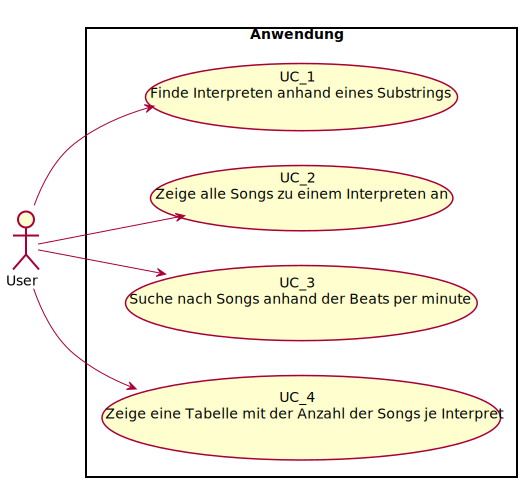
\includegraphics[width=0.5\textwidth]{images/useCaseDiagramm.png}
	\caption{Anwendungsfall-Diagramm, UML 2.0. Alle Anwendungsfälle für das Million-Song-Projekt}
	\label{anforderungen:usecasediagramm}
\end{figure}

Es folgt eine kurze Beschreibung der einzelnen Anwendungsfälle. Auf eine detaillierte Ausarbeitung im Rahmen einer 
ausführlichen Anforderungsanalyse soll in diesem Falle verzichtet werden, weil ein konkretes Anwendungsszenario fehlt und
die Anwendungsfälle künstlicher Natur sind, um den Einsatz von Hadoop, MapReduce und Hbase im Bereich der
Big-Data-Anwendungen zu evaluieren.

\begin{description}
	\item[UC 1] Der Nutzer möchte den Namen aller Musikstücke, die ein bestimmter Interpret geschrieben hat.
	\item[UC 2] Der Nutzer möchte für sein Lauftraining nur den Namen jener Musikstücke haben, die eine Beats-Per-Minute-Rate
		von 120 haben.
	\item[UC 3] Der Nutzer möchte den Namen aller Musikstücke, die länger als 5 Minuten am Stück laufen.
	\item[UC 4] Der Nutzer möchte ein oder mehrere Musikstücke eines bestimmten Namens. Dabei muss der Name nicht dem 
		kompletten Musiktitel beschreiben.
	\item[UC 4] Der Nutzer möchte die Namen aller Musikstücke erhalten, die in einem bestimmten Jahr zum ersten Mal erschienen sind.
\end{description}

\subsubsection{Rahmenbedingungen}
Die Rahmenbedingungen teilen sich in die Hardware-Rahmenbedingungen und in die Software-Rahmenbedingungen auf.
Die Hardware, die uns zur Verfügung gestellt wurde besteht aus einem Verbund von 5 homogenen Server-Rechnern, 
die über ein Ethernet-Netzwerk gleichwertig miteinander verknüpft sind. Physikalisch sind alle Knoten an einem gemeinsamen
Switch angeschlossen als physikalische Stern-Topologie. Dies hat aus logischer Sicht zur Folge, dass eine direkte Kommunikation
zwischen den Knoten möglich ist. Die Bandbreite des gesamten Netzwerkes ist mit 20Mbit/s angegeben, was durch die Topologie
auch zwischen den einzelnen Knoten möglich wäre.

Die Server-Knoten sind alle mit folgender Hardware ausgestattet:
\begin{itemize}
	\item Intel i7-4790K CPU
	\item 32 GB RAM
	\item 256 GB SSD
	\item 2 TB HDD
\end{itemize}

Auf der Seite der Software ist auf allen Knoten mit \textit{Ubuntu} eine Linux-Distribution in der Version 
\textit{16.04.1 LTS Server 64-Bit} installiert. Root-Rechte sind gewährt.
Anzumerken ist, dass alle Ressourcen mit 9 anderen Teams geteilt werden und alle Teams auf der selben 
Instanz des Betriebssystems arbeiten und nur durch unterschiedliche Nutzer getrennt sind. 
Diese Rahmenbedingung ist insbesondere bei der Konfiguration der Netzwerk-Ports bei verteilten Anwendungen 
zu beachten, da verschiedene Anwendungen eventuell auf dem gleichen Port lauschen und somit 
Konflikte entstehen können.

\subsubsection{Installation und Konfiguration}
Auf dem Cluster wird das komplette Hadoop-Softwarepaket installiert, bestehend aus den
Komponenten \ac{YARN}, \ac{HDFS} und MapReduce. Installiert wird über einen Tarball von der offiziellen
Apache-Webseite (\url{http://www-us.apache.org/dist/hadoop/common/hadoop-2.7.3/hadoop-2.7.3.tar.gz}), um die aktuellste Version ($2.7.3$) von Hadoop zu erhalten. Die Installation selbst gestaltet sich mit dem entpacken der binär-Dateien im home-Verzeichnis 
denkbar einfach. Komplexer gestaltet sich die Konfiguration, die das Laufzeitverhalten der Komponenten festlegen.

Die folgenden Tabellen zeigen die Konfiguration der einzelnen Hadoop-Komponenten, die vom der Standard abweicht.
Eine Auflistung der ab Werk ausgelieferten Standard-Konfiguration kann auf folgenden Webseiten nachgeschlagen werden:
\cite{hdfsDefault}, \cite{yarnDefault} und \cite{mapreduceDefault}.


\subsection{Implementierung von MapReduce-Funktionen}

Dieser Abschnitt beschreibt die Implementierung von Map-Reduce-Funktionen, die auf den Daten
des Million-Song-Datensatzes arbeiten. Vorausgesetzt wird, dass der Million-Song-Datensatz als
CSV-Datei bereit in das HDFS-Dateisystem importiert ist. Die hier vorgestellten MapReduce-Funktionen
arbeiten ausschließlich mit Daten auf dem HDFS-Dateisystem, abgesehen von den Zwischenergebnissen,
die auf dem lokalen Dateisystem des jeweiligen Knotens abgelegt werden.
Für die Implementierung wird die Java-API des MapReduce von Hadoop verwendet. Wichtig ist,
dass die aktuelle MapReduce-API verwendet wird, und nicht die inzwischen veraltete MapRed-API.
Eine gute Hilfe bei der Entwicklung von map- und reduce-Funktionen bietet \cite{miner2012mapreduce}.

Die erste Implementierung der MapReduce-Funktionen überführt alle Songs aus der ursprünglichen
CSV-Datei in eine neue CSV-Datei, in der erstens kein Song mehr doppelt vorkommt und zweitens
ein Song nur noch eine Untermenge der ursprünglichen Attribute enthält. Damit soll der ursprüngliche
Datenbestand auf einen reduzierten Datenbestand mit den für den Nutzer interessanten Attributen 
transformiert werden. Die map-Funktion ist dafür verantwortlich, die Attribute eines Musikstückes
zu identifizieren und daraus mit einen neuen Musikstück-Eintrag zu erzeugen, der nur noch die interessanten
Attribute enthält.
Zuerst muss definiert werden, welche Eingabeparameter die map-Funktion bekommt. Dazu gibt es verschiedene
Eingabeformate der MapReduce-API, unter denen man wählen kann. Weil die Daten in der CSV-Datei für das
MapReduce-Framework nichts weiter als reiner Text ist, wird das \textit{Text}-Format als Eingabe für
die map-Funktion gewählt, welches gleichzeitig auch das Standard-Format für die map-Funktion ist.
Das Format des Schlüssel-Parameters wird nicht weiter angegeben, weil der Schlüsselwert in diesem Falle 
während der Verarbeitung keine Rolle spielt.
Die map-Funktion teilt den übergebenen Wert des Textes in die Song-Attribute auf, indem es den Text
als einzelnen String betratet und mittels der \textit{split}-Methode ein Feld von String erzeugt, die durch
das Komma im String getrennt sind. Dadurch sind die Musik-Attribute als Strings nun einzelnen verfügbar.
Der neue Eintrag für den Song wird durch das Erzeugen eines neuen Strings und dem Anhängen ausgewählter
Attribute erzeugt. Ist der neue String fertig zusammen gebaut, wird er wieder in das hadoop-spezifische \textit{Text}
konvertiert und als Zwischenergebnis dem MapReduce-Framework übergeben. Dieses erwartet neben dem 
Wert aber auch einen Schlüssel. Der Schlüssel ist in dem Falle ebenfalls vom Typ \textit{Text}, der als Wert die
Song-ID des Musikstückes enthält.

\lstset{
    language=Java,
    basicstyle=\ttfamily,
    frame=single,
    breaklines=true,
    postbreak=\raisebox{0ex}[0ex][0ex]{\ensuremath{\hookrightarrow\space}}
}

\begin{lstlisting}
  protected void map(Object key, Text value, Context context) {
      String[] allAttributes = value.toString().split(",", maxNumOfAttr);
      String newStrippedValue = new String();
      songId.set(allAttributes[songIdColumn-1]);
      
      for(int i=0; i<untilGenreAttr; i++){
          newStrippedValue += ","+allAttributes[i];
      }
      
      for(int k=fromGenreAttr-1; k<maxNumOfAttr; k++){
          newStrippedValue += ","+allAttributes[k];
      }
      
      strippedSongAttr.set(newStrippedValue);
      context.write(songId, strippedSongAttr);
   }
\end{lstlisting}

%\usepackage{listings}
\subsubsection{Import der Daten}
Um die Verwendung von der NoSQL Datenbank HBase und das Programmiermodel MapReduce zu demonstrieren greifen wir auf die frei verfügbare Liste der Daten zu, die millionen Datensätze zu den verschiedenen Liedern enthält. Die Datensätze werden vom Fachbereich (????) bereitgestellt und sind in dem Verzeichnis "/data/team6/MillionSongSubset/data" in den *.h5 Dateien zu finden. 

Unsere erste Aufgabe lag darin die Daten aus den *.h5 Dateien in die HBase Datenbank zu importieren.
Dafür verwenden wir Java Bibliothek "ncsa.hdf.object.h5". Mit Hilfe dieser Bibliothek können wir auf die einzelnen Spalten innerhalb der H5 Datei zugreifen.
Nachdem wir die Tabelle 'Music' in HBase DB erstellt haben, haben wir uns üäber die Struktur der Tabelle Gedanken gemacht. Dabei fiel uns auf, dass wir für unsere UseCases nicht alle Spalten brauchen würden und somit wir zwei Spaltenfamilien erstellen könnten Somit entstanden zwei Spaltenfamilien "song" und "miscellaneous". In der Spaltenfamilie "song" haben wir zusätzliche Spalten erstellt, um die Suche nach den Daten zu vereinfachen. In der Spaltenfamilie "miscellaneous" haben wir eine große Spalte erstellt, die alle restlichen Daten beinhaltet, die mit voneinander mit Semicolon getrennt sind.
Dadurch, dass wir eigenes Java Programm für den Import der Daten implementiert haben, konnten wir die Daten in die richtige Spaltenfamilie verteilen.

Im folgenden zeigen wir ein paar Codefragmente zu unserem Datenimport:

Zuerst müssen wir eine Connection zum HBase aufbauen:

%\begin{lstlisting}[language=bash]
%  $ wget http://www-us.apache.org/dist/hbase/stable/
%    hbase-1.2.4-bin.tar.gz
%  $ tar -xzf hbase-1.2.4-bin.tar.gz
%  $ ln -s hbase-1.2.4 hbase
%  $ cd hbase
%  $ export PATH=$PATH:~/hbase/bin
%\end{lstlisting}


\begin{lstlisting}[language=Java]
Configuration config = HBaseConfiguration.create();
            config.setInt("timeout", 120000);
            config.set("hbase.master", "*" + hbaseHost + ":16006*");
            config.set("hbase.zookeeper.quorum","10.20.110.61");
            config.set("hbase.zookeeper.property.clientPort", "2186");
	   Connection connection = ConnectionFactory.createConnection(config);
\end{lstlisting}

Nachdem wir eine Verbindung zur Datenbank haben können wir die Tabelle "music" holen:

\begin{lstlisting}[language=Java]
Table table = connection.getTable(TableName.valueOf("music"));
\end{lstlisting}

Eine Datenreihe erzeugen wir mit dem Put-Object:

%\begin{lstlisting}[language=Java]
Put p = new Put(Bytes.toBytes("Song1"));
/*Erzeugen ein Datensatz mit dem RowKey = "Song11''*/
\\p.addColumn(Bytes.toBytes("song"), Bytes.toBytes("Title"),Bytes.toBytes("HISTORY"));
/*Erzeuge für diesen RowKey in der Spaltenfamilie "song", Spalte: "Title" den Wert "HISTORY"*/
\\table.put(p);
%\end{lstlisting}
\subsection{crud_operationen}
\subsection{client_impl}
%Beiden letzten Kapitel stehen zur Disposition
\subsection{HBase-Tuning}
\subsection{Benchmark-Tests}

%\chapter{Hadoop}
\cite{Wartal2012}
\cite{Endlich2011}
\section{Einleitung}
\section{Das HDFS-Dateisystem}
\section{Das MapReduce-Framework}
\section{Module für Hadoop}

\newpage

% loads the fancy pagestyle for register part
%\input{fancyRegisterPart}

% #####
% # load the appendix from the files
% #####
\input{appendix}

% #####
% # list of table, list of figures, and list of listings in ToC
% #####
%\newpage
%\addcontentsline{toc}{chapter}{Abbildungsverzeichnis}
%\listoffigures
%\newpage
%\addcontentsline{toc}{chapter}{Tabellenverzeichnis}
%\listoftables
%\newpage
%\addcontentsline{toc}{chapter}{Listings}
%\lstlistoflistings

% #####
% # List of Abbreviations
% #####

%\phantomsection 
%\addcontentsline{toc}{chapter}{Abkürzungsverzeichnis}
%\renewcommand\refname{Abkürzungsverzeichnis} 
%\chapter*{Abkürzungsverzeichnis}
%\input{abbreviations}
%\newpage

% #####
% # load the bibliography
% #####
%Quelle: http://dbs.uni-leipzig.de/file/seminar_1112_gharib_ausarbeitung.pdf
%http://stackoverflow.com/questions/16929832/difference-between-hbase-and-hadoop-hdfs
\bibliography{bibliography}

% #####
% # load the sworn declaration
% #####
\input{declaration}
%\input{chapter1}
% end of the document
\end{document}
